\chapter{Side projects}

\section{Healthcare-Network}

\begin{figure}[H]
    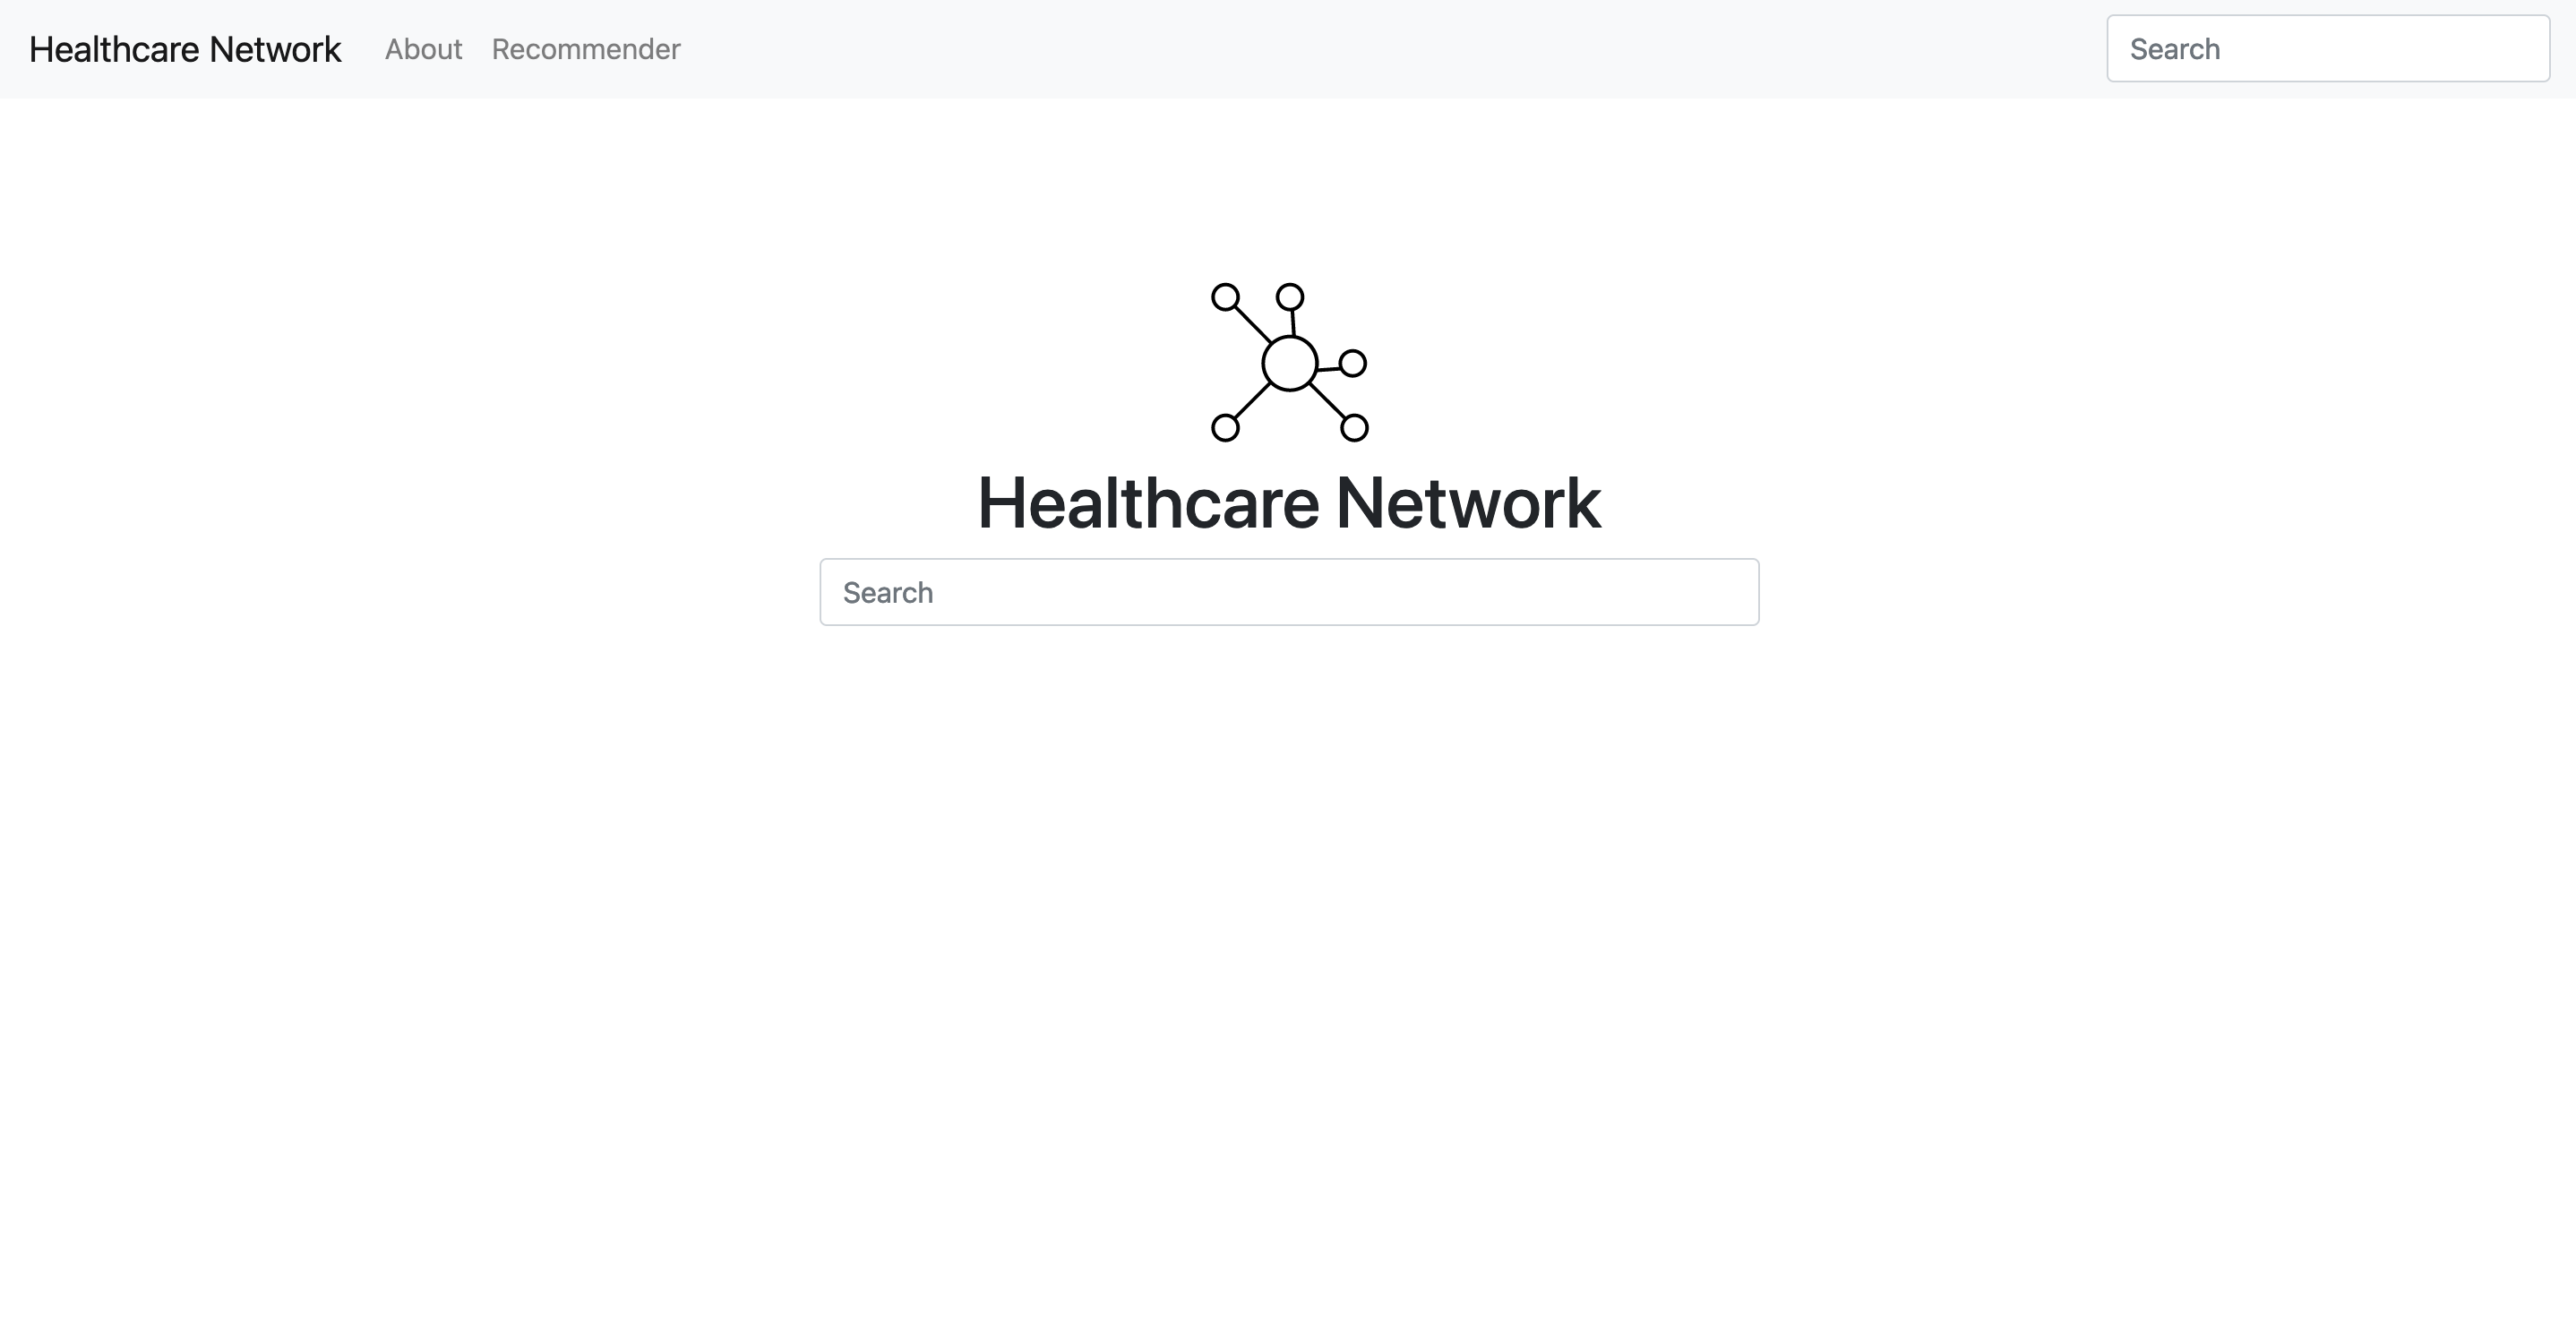
\includegraphics[width=0.7\textwidth]{images/healthcare-network/home.png}
    \centering
    \caption{
        Healthcare-Network: homepage. A minimalist page with a search bar allowing to find hospitals based on their name, category, or location.
    }
    \label{fig:hn-home}
\end{figure}


\begin{figure}[H]
    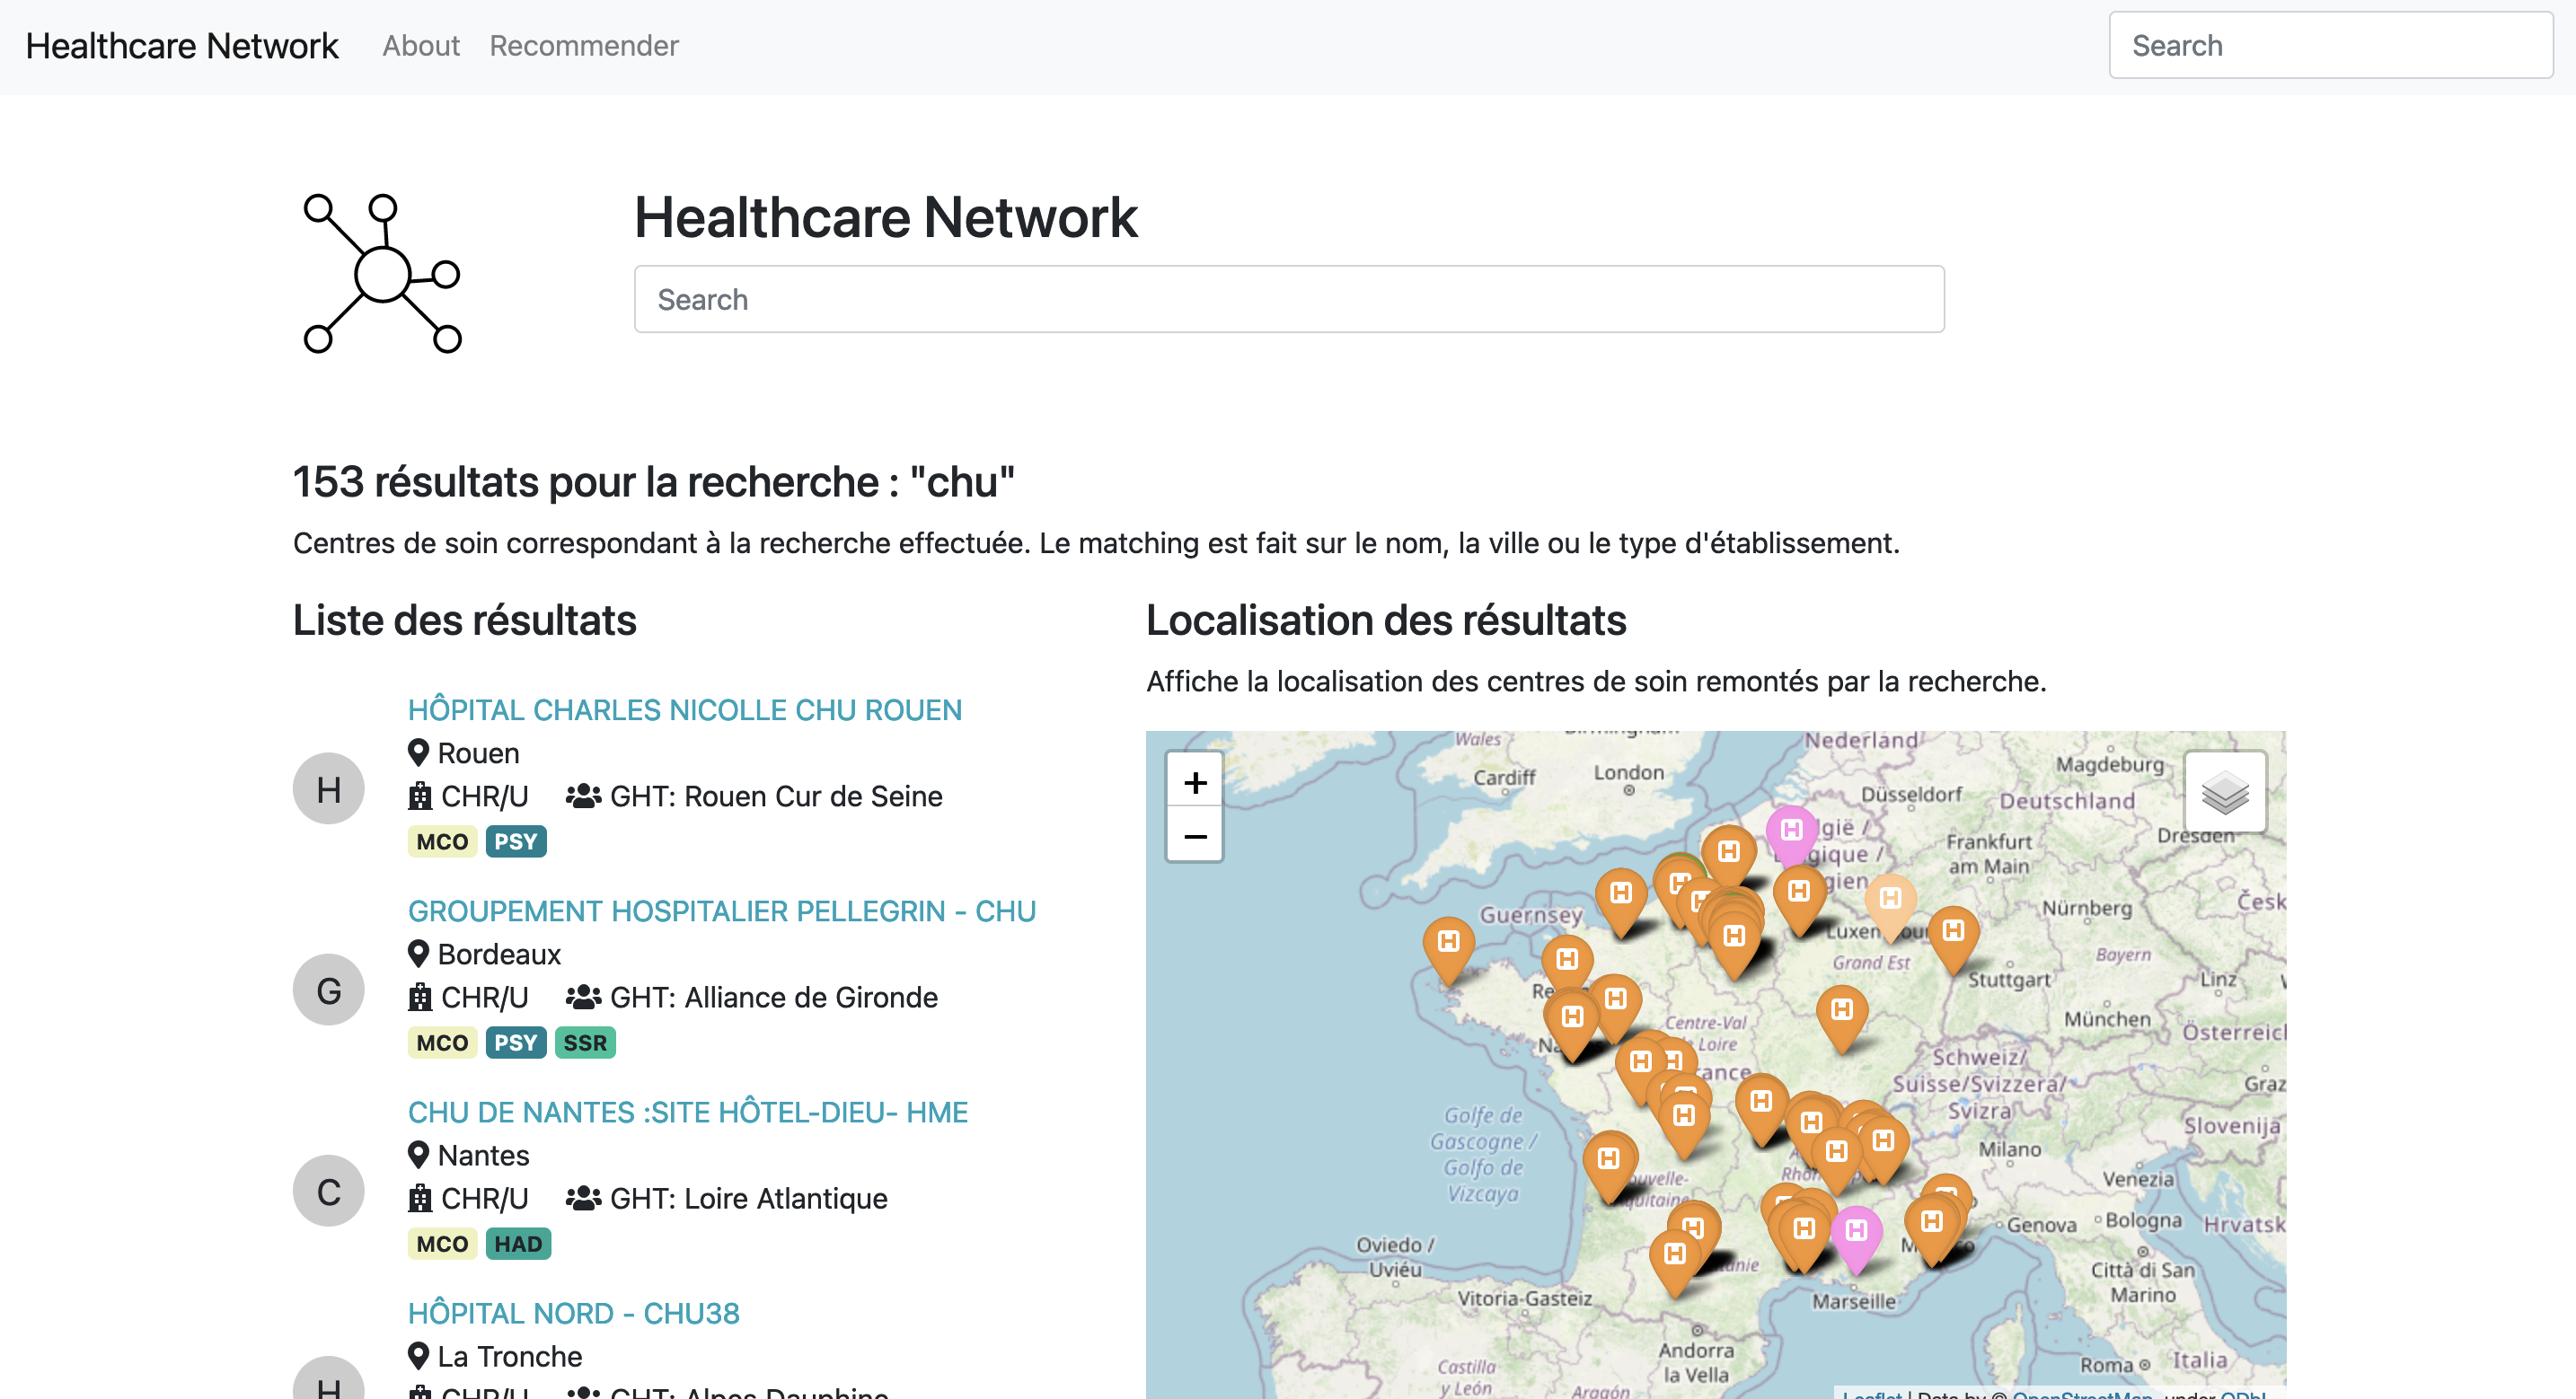
\includegraphics[width=0.7\textwidth]{images/healthcare-network/search.png}
    \centering
    \caption{
        Healthcare-Network: search results. The list of retrieved hospitals and their details is displayed, as their position on a map. This query shows all the \ac{chru} hospitals in metropolitan France.
    }
    \label{fig:hn-search}
\end{figure}


\begin{figure}[H]
    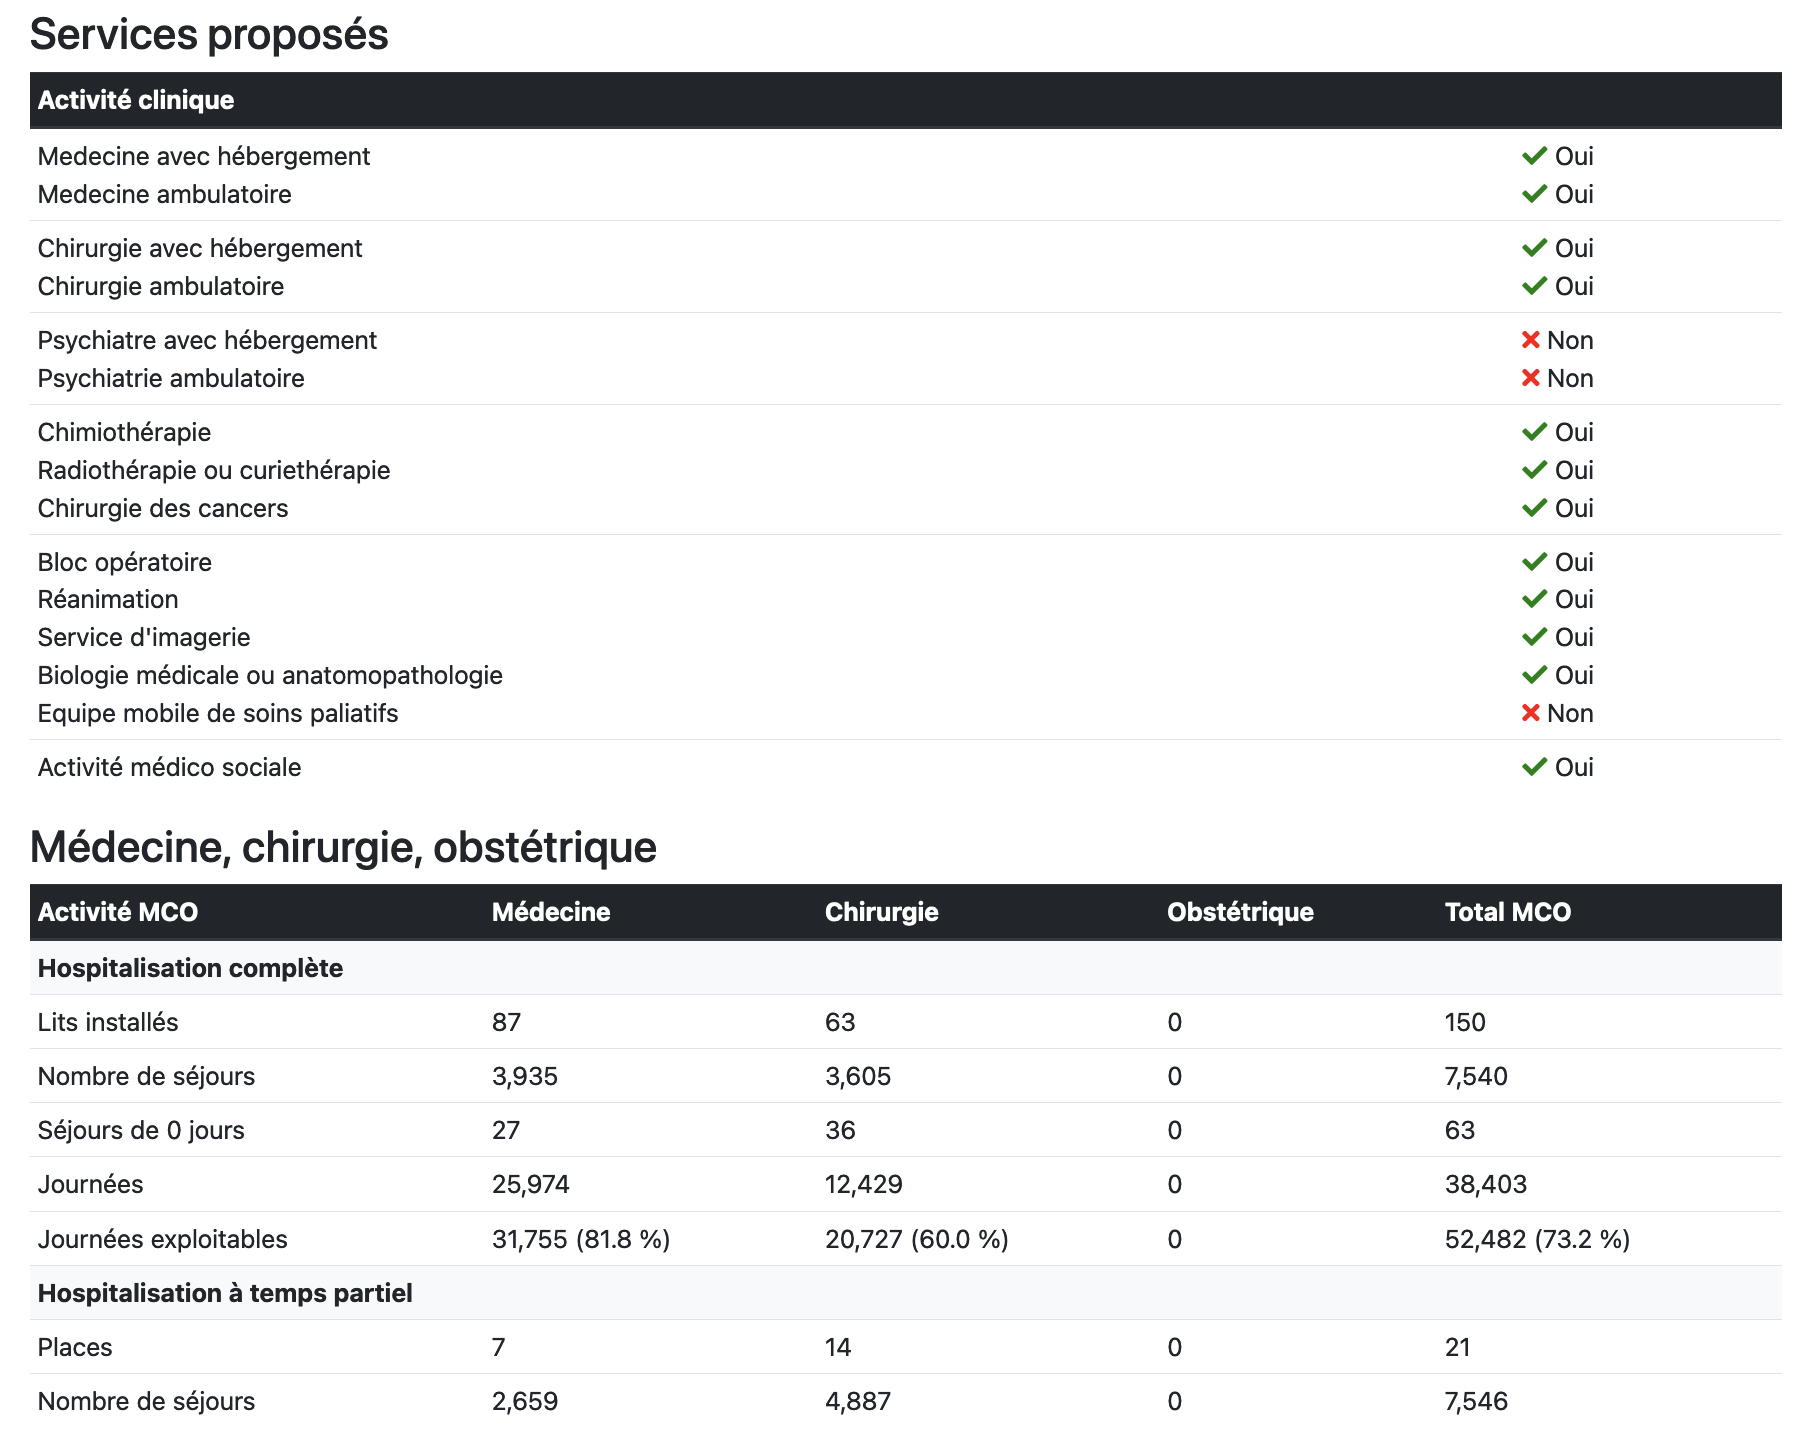
\includegraphics[width=0.7\textwidth]{images/healthcare-network/curie-services.png}
    \centering
    \caption{
        Healthcare-Network: description of health services offered, and statistics on \ac{mco} activity for Institut Curie Paris hospital.
    }
    \label{fig:hn-curie-services}
\end{figure}


\begin{figure}[H]
    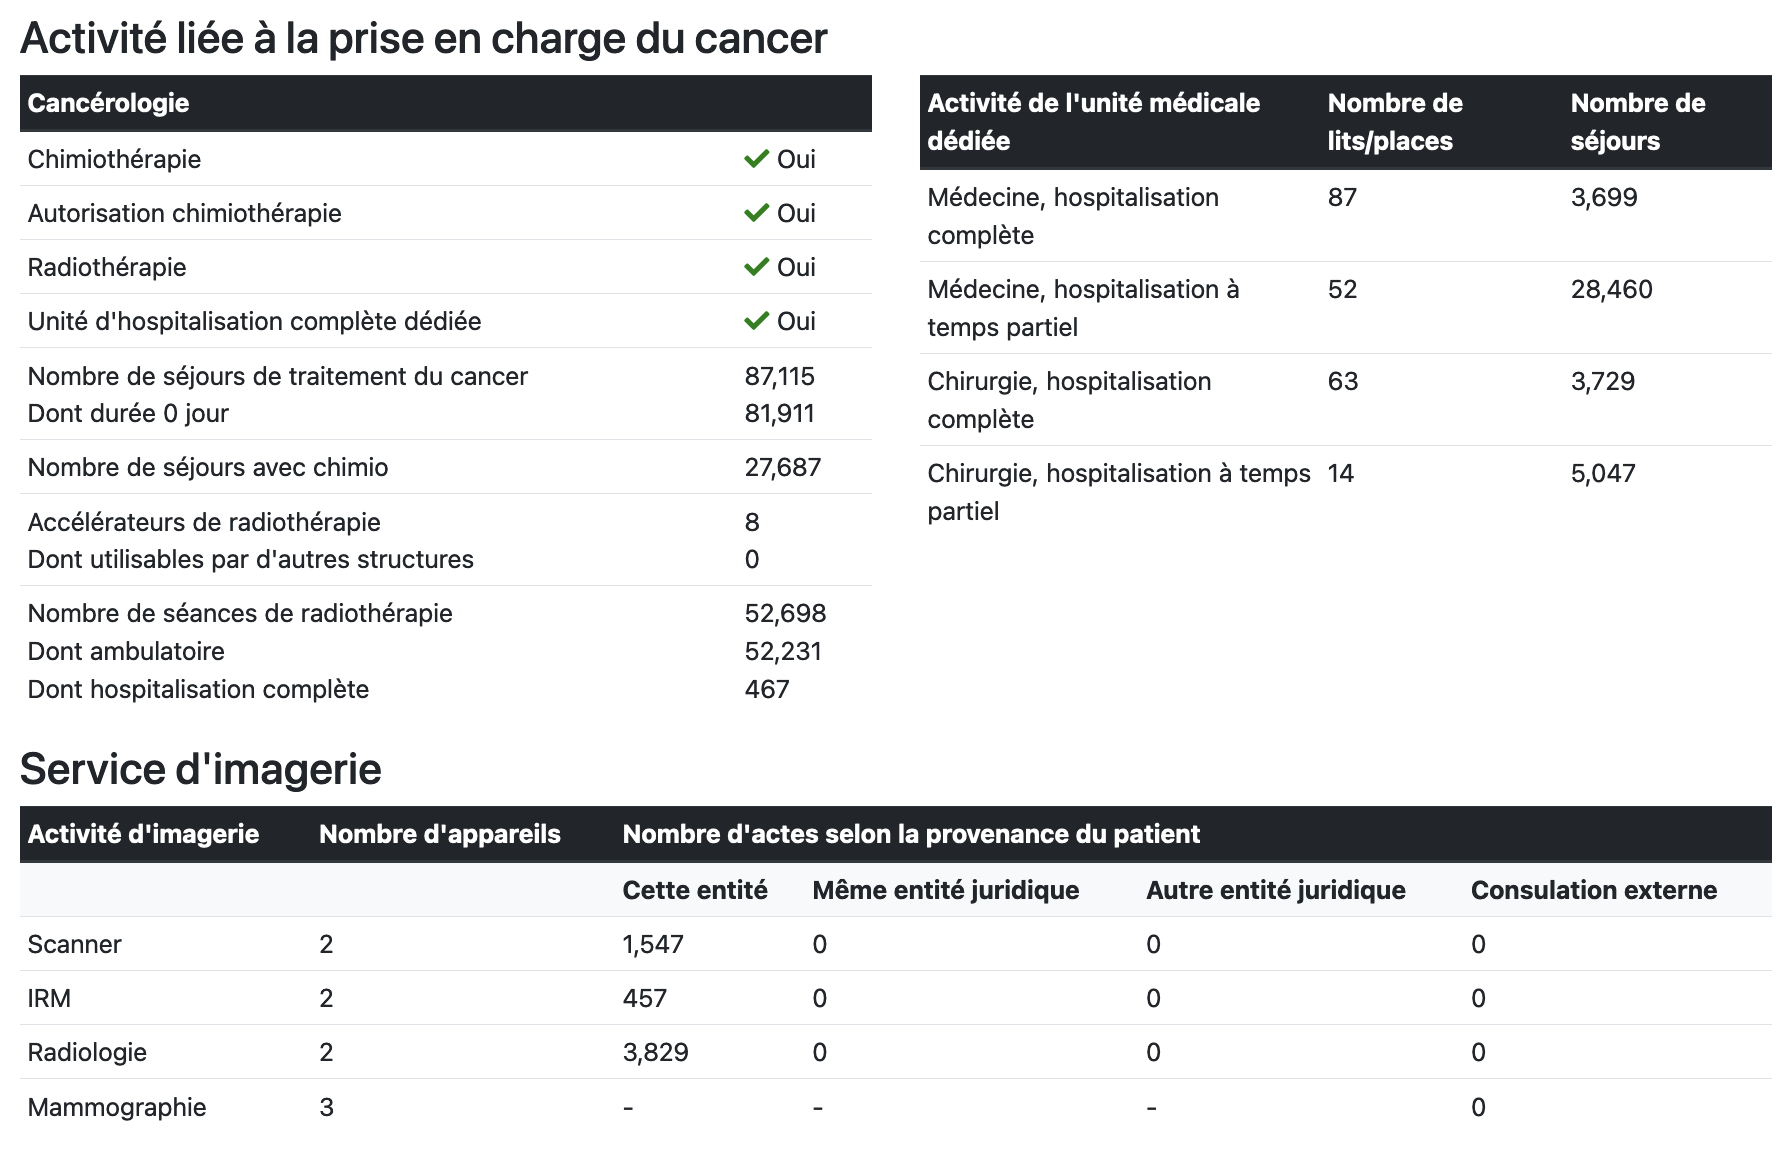
\includegraphics[width=0.7\textwidth]{images/healthcare-network/curie-cancero.png}
    \centering
    \caption{
        Healthcare-Network: description of oncology activity for Institut Curie Paris hospital.
    }
    \label{fig:hn-curie-cancero}
\end{figure}


\begin{figure}[H]
    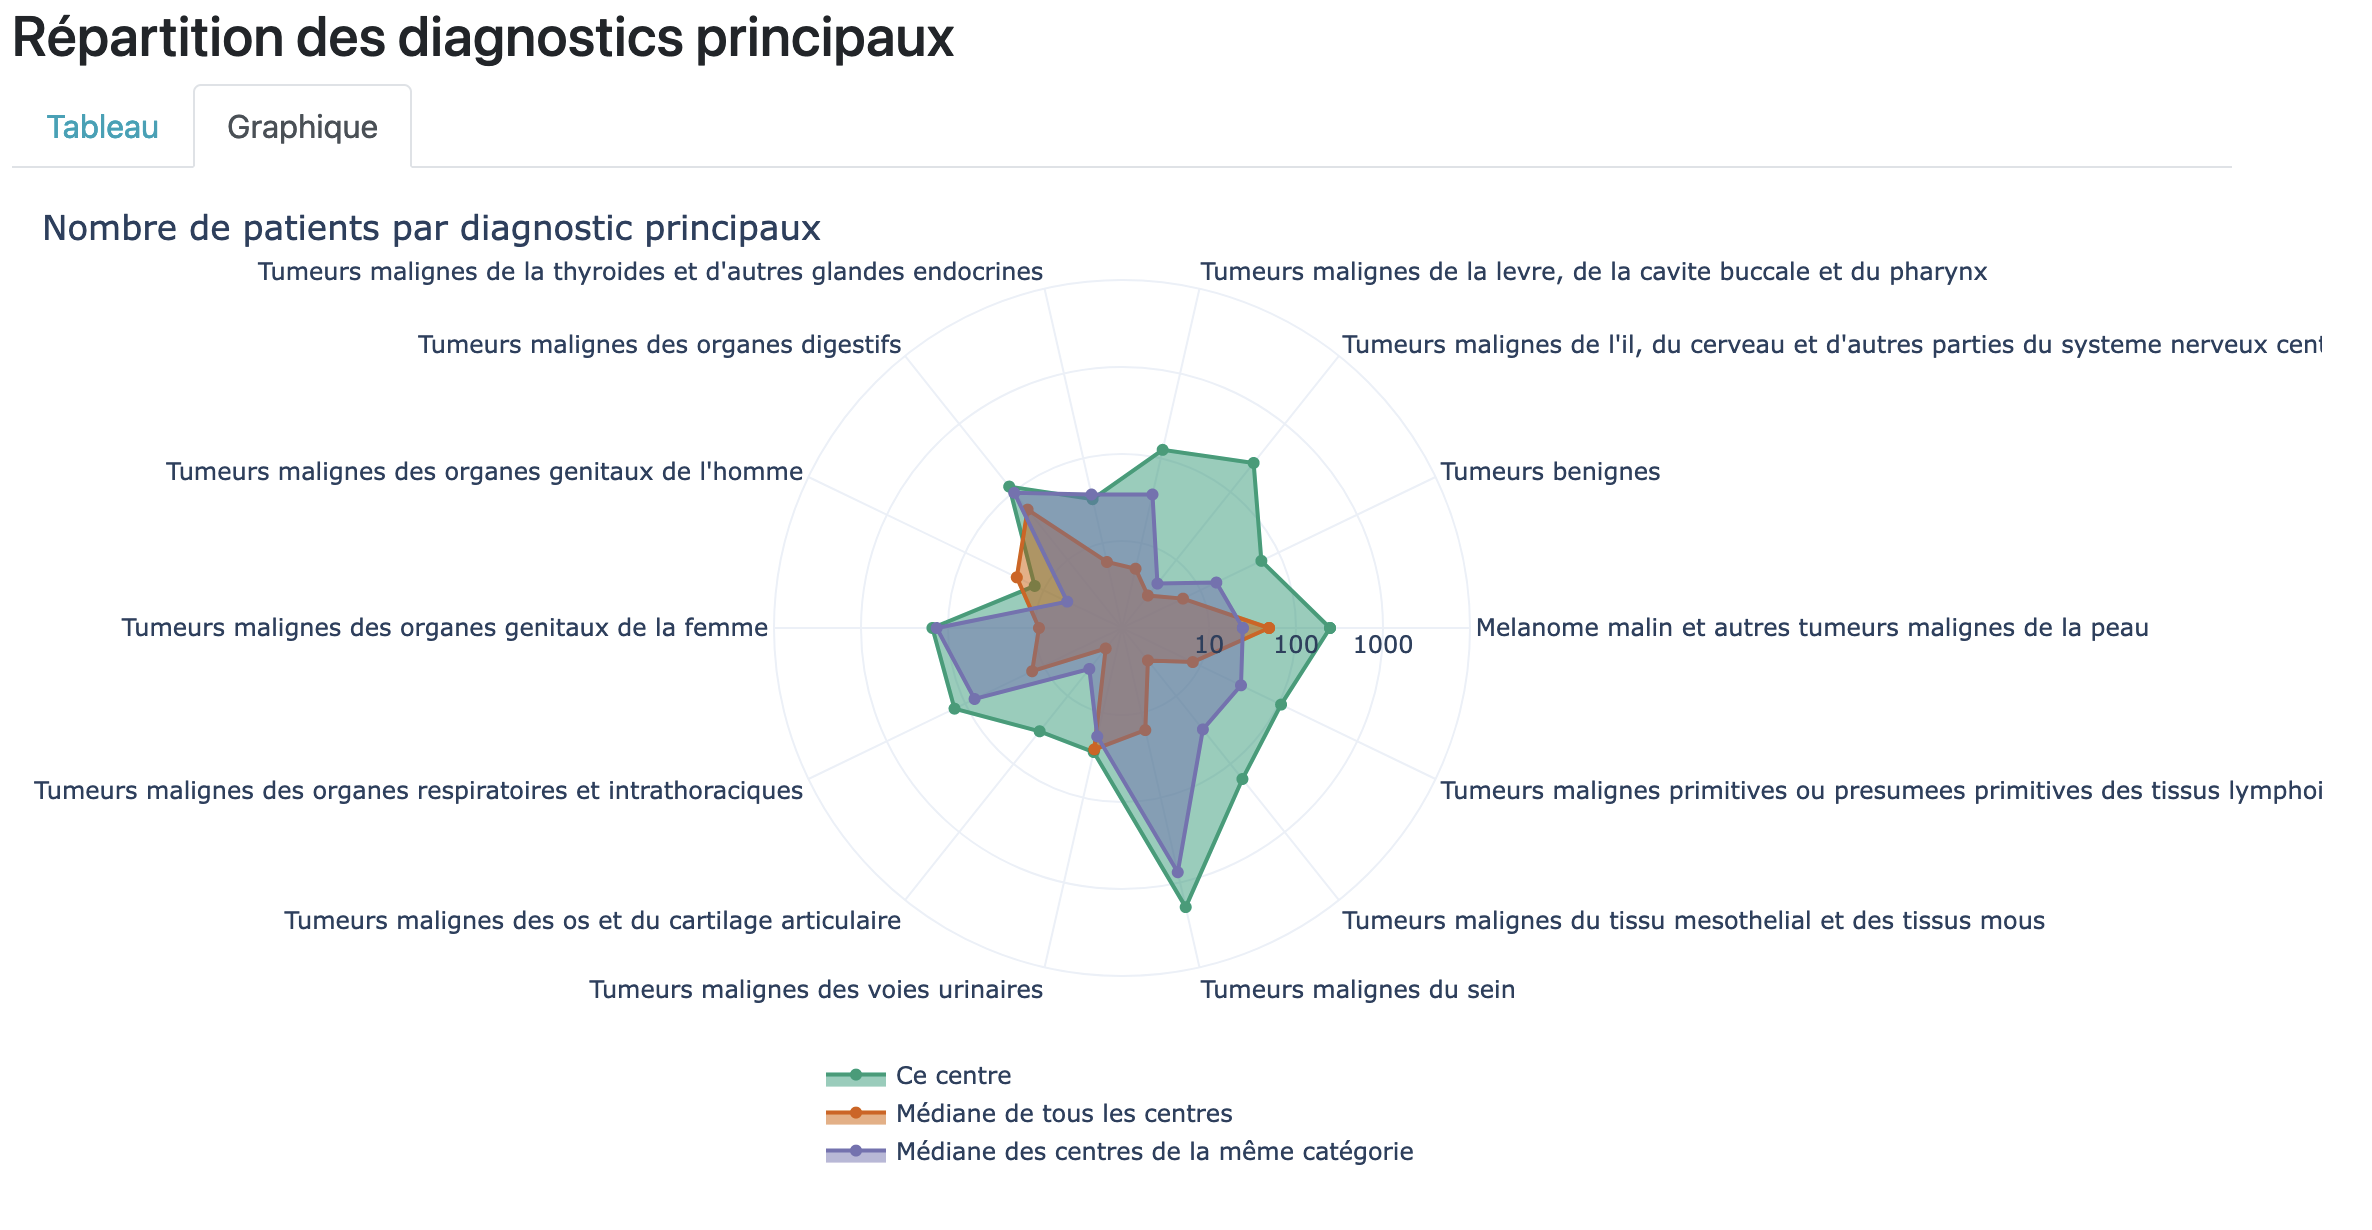
\includegraphics[width=0.7\textwidth]{images/healthcare-network/curie-dp.png}
    \centering
    \caption{
        Healthcare-Network: number of patients per cancer related diagnosis for Institut Curie Paris hospital. Comparison with the median statistics from hospitals within the same category (\ac{clcc}) and overall median.
    }
    \label{fig:hn-curie-dp}
\end{figure}


\begin{figure}[H]
    \includegraphics[width=0.7\textwidth]{images/healthcare-network/curie-co-occ.png}
    \centering
    \caption{
        Healthcare-Network: map of the hospitals that have the most co-occurrences with Institut Curie Paris. Co-occurrences between two hospitals are defined as the number of patients who visited both hospitals during their care pathways. To illustrate facility attractiveness, municipalities are colored by the number of inhabitants who visited the Institut Curie Paris hospital.
    }
    \label{fig:hn-curie-co-occ}
\end{figure}


\begin{figure}[H]
    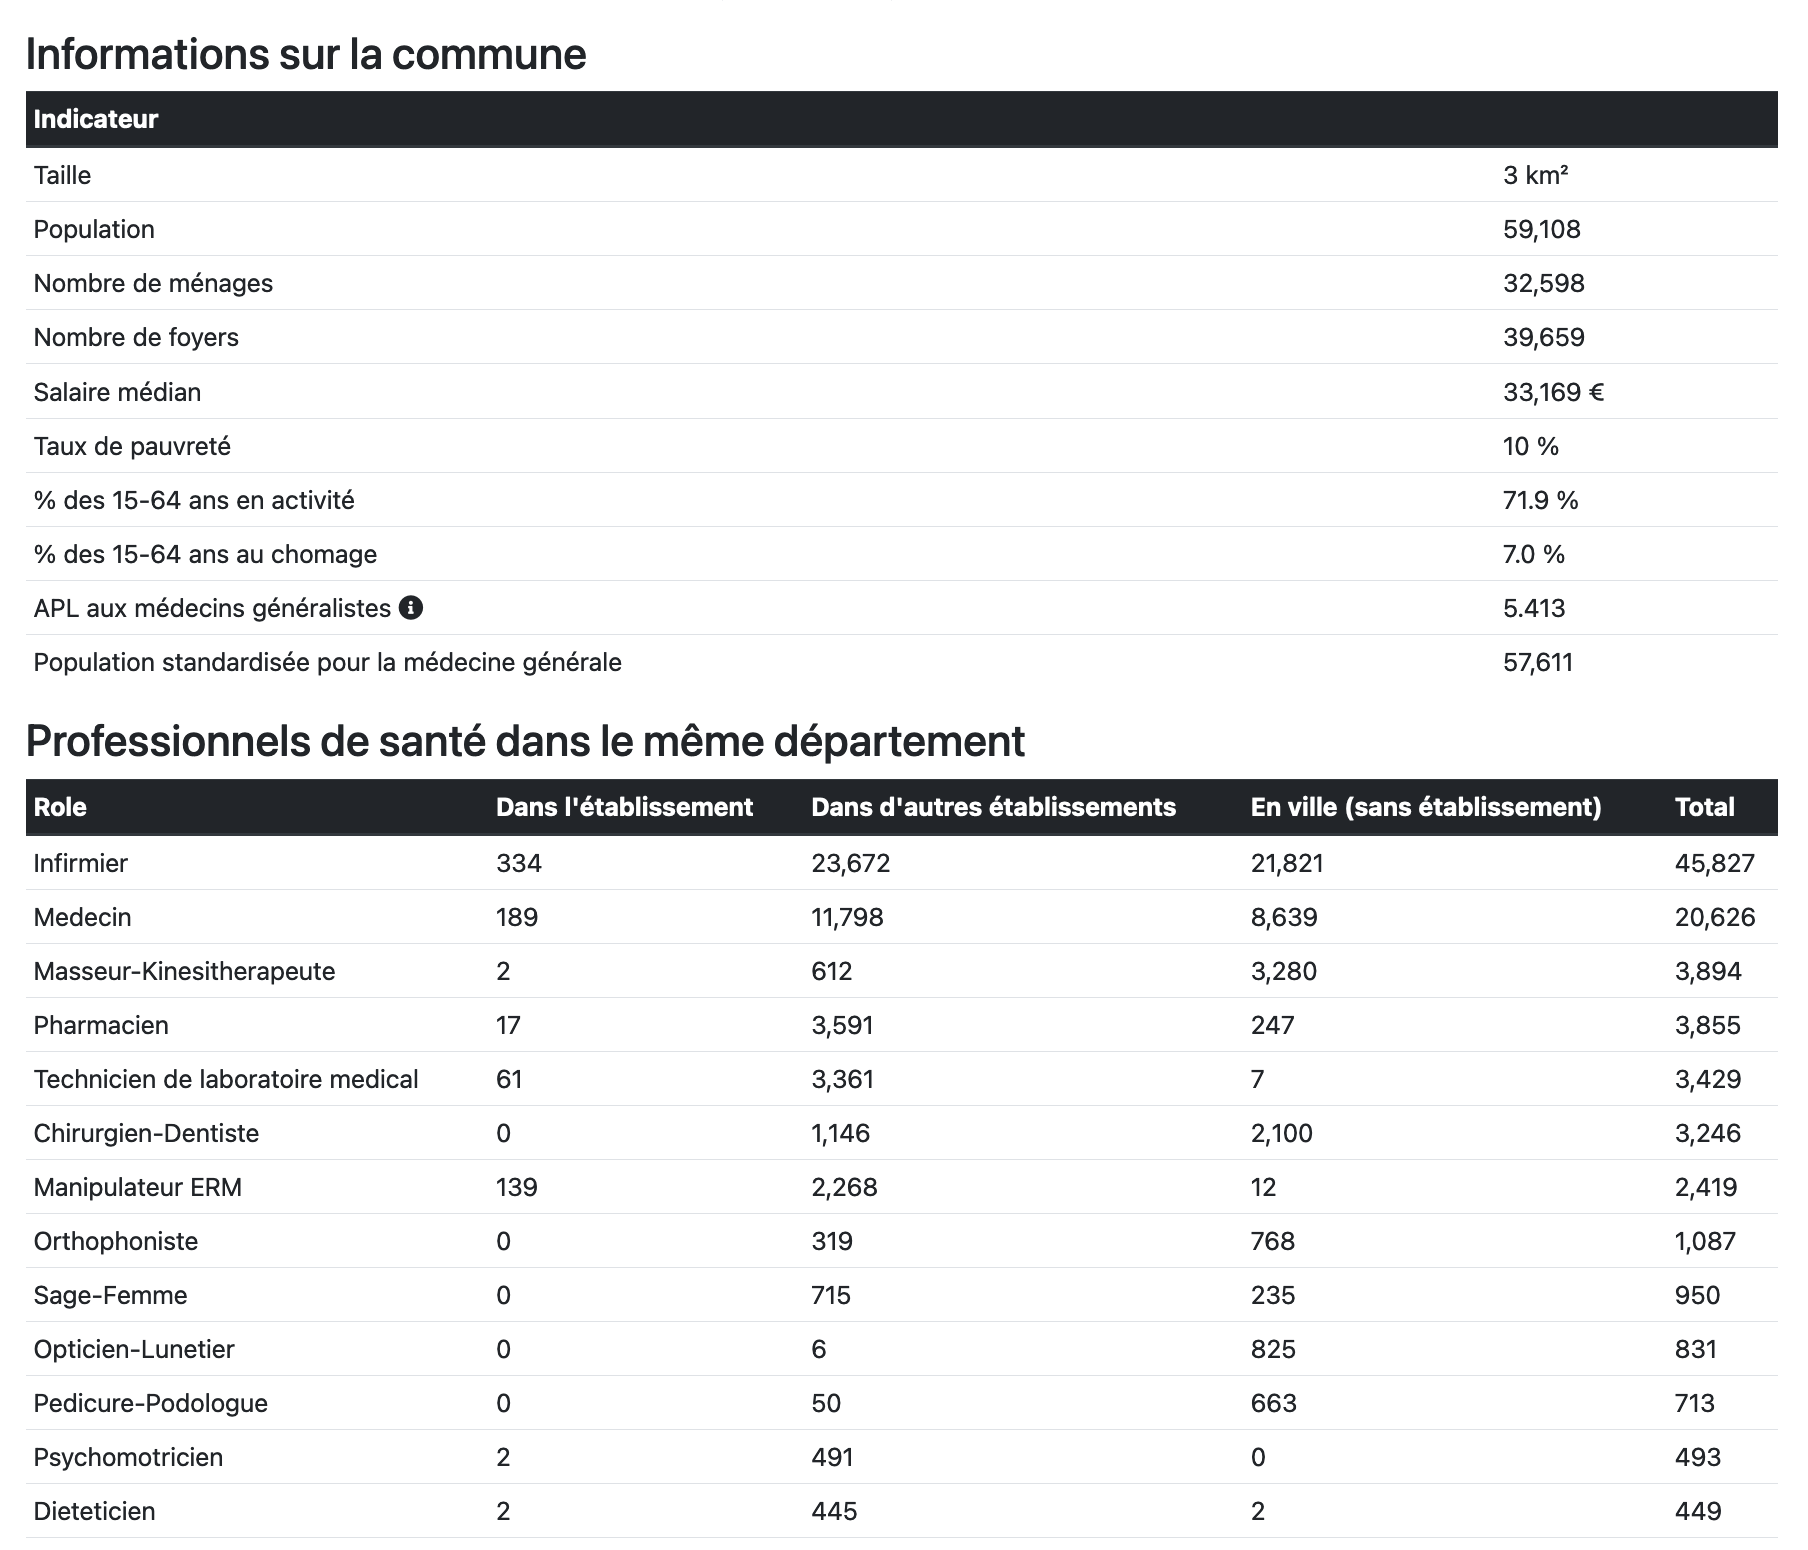
\includegraphics[width=0.7\textwidth]{images/healthcare-network/curie-commune.png}
    \centering
    \caption{
        Healthcare-Network: statistics on the municipality where Institut Curie Paris is located (Paris 75105). Population, median salary and accessibility to primary care are displayed to qualify the hospital neighborhood. Health professionals within the department are also listed to illustrate the health supply available around the hospital.
    }
    \label{fig:hn-curie-commune}
\end{figure}


\section{Affiliation Generator}

Affiliation Generator is a web application that helps you manage your papers authors and their affiliations. The app will let you upload a list of researchers from your team, as well as their affiliations. When you're writing a new paper, simply drag and drop authors in the required order of authorship and the app will generate the list of authors to copy-paste in your paper.

You can edit your researchers and institutions list. Every researcher can be attached to one or many institutions. The generator page will let you drag and drop researchers in the order of authorship on your paper. Once your click generate, the app will retrieve the affiliations from your researchers and format them automatically for you so that you only have to copy paste this into your paper. You can also create papers, drag and drop the authors in the order you want, save them and add more authors later.

The application is deployed within Institut Curie at the following address:

\url{https://affiliation-generator.curie.net/}.
